\documentclass[letterpaper, 10 pt, conference]{IEEEconf}

\usepackage{fancyhdr}
\usepackage{amsmath,amsfonts,graphicx}
\usepackage{cite}
\usepackage{caption}
\usepackage{siunitx}
\usepackage{natbib}
\usepackage{url}
\usepackage{listings}
\usepackage{hyperref}
\fancyhf{} % clear all header and footers
\renewcommand{\headrulewidth}{0pt} % remove the header rule
\cfoot{\thepage}
\captionsetup[figure]{font=normalsize,labelfont=bf}
\setlength{\footskip}{45pt}
\title{\LARGE \bf
Enabling Concurrent Ambient Backscatter Communications in Multipoint-to-Point Topologies
}


\author{Andr{\'e} Monteiro, Jared Weinstein, R.I. Zelaya\\
Yale University\\
\{andre.monteiro, jared.weinstein, rotman.zelaya\}@yale.edu
}

\providecommand{\keywords}[1]{\textbf{\textit{Key Words---}} #1}

\pagestyle{fancy}
\begin{document}

\nocite{*}

\maketitle
\thispagestyle{fancy}
\pagestyle{fancy}



\begin{abstract}

This paper introduces two mechanisms to decode simultaneous ambient backscatter communications in a multipoint-to-point topology. We model a network where two independent wireless nodes attempt to communicate concurrently with the same receiver by backscattering an arbitrary AM signal. We present the operation of our algorithms by implementing the aforementioned network in GNU Radio Companion. We argue that, given the right conditions, our decoding procedures allow a receiver to decode simultaneous ambient backscatter transmissions with an acceptable Bit Error Rate. To the best of our knowledge, this is the first work that studies multipoint-to-point concurrent backscatter communications. 

\end{abstract}
\keywords{Ambient Backscatter; Wireless Communications; Modulation and Demodulation.}


\section{INTRODUCTION}

Low-powered wireless devices are becoming increasingly pervasive in modern communication infrastructures. The proliferation of the IoT (Internet of Things) has propelled the integration of wireless systems in what could be considered unusual places, such as books, thermostats, and even the human body \cite{jang2016stent}. As these devices become smaller and more numerous, a clear challenge is how to power them. Incorporating wires and/or batteries on these devices is clearly an unfeasible solution. Just imagine how uncomfortable it would be to have wires running all over your body just to measure your glucose level.

A clever solution to the power-delivery problem was proposed by Smith et al. in their seminal paper on ambient backscatter \cite{liu2013ambient}. In short, their solution allows two battery-free devices to communicate with each other by backscattering (i.e., reflecting) ambient TV signals. A device transmitting information switches between reflecting and non-reflecting states to convey (modulate) either a "1" or a "0" bit, respectively. The backscattering is done at a much lower data rate than the ambient signals so that the receiver can demodulate the information through averaging. By reusing generic ambient signals, the devices have no need to generate their own carrier waves, which in turn means that no energy source other than the exogenous signals is required.

In this paper, we ask the following question: can a receiver in a backscatter network decode two simultaneous data streams through Layer 1 algorithms? More generally, we address the challenge of demodulating concurrent transmissions in a multipoint-to-point ambient backscatter network. We propose two decoding mechanisms. The first one, which we call \textit{Demodulation via Power Superposition}, discovers the possible power levels of the sum (superposition) of the signals sent individually and independently by each transmitter. Each power level represents a sequence of of bits, one bit for each transmitter. The second solution, which we call \textit{Demodulation via Time Offset}, works by allowing one of the data streams to be ahead of the other. Power estimations are performed at specific time intervals to determine which bit and which transmitter were involved in the signal's power fluctuation. We specify under which assumptions these algorithms work, as well as the pros and cons of each approach. We simulate the topology of interest and test the performance of our decoding mechanisms in GNU Radio Companion.

The remainder of this paper is organized as follows. In Section 2 we describe the physical conditions under which we assume our simulated network operates. We calculate the estimated power of the AM signal that the devices involved receive and present all the relevant assumptions. In Section 3 we describe the mechanisms used by the backscatterers in our simulation to transmit information. In Section 4 we present our demodulation algorithms as well as the benefits and setbacks of each. We evaluate the performance of these algorithms in Section 5 and derive conclusions in Section 6.

\section{SCENARIO OF INTEREST}

Figure 1 illustrates the scenario under consideration. We study a multipoint-to-point topology in which $B_1$ and $B_2$ attempt to communicate simultaneously with $R$ by backscattering an arbitrary AM signal. Our model positions the AM transmitter 6.47 kilometers away from the backscatterers and the receiving node. This is the approximate distance between the Arthur K. Watson Hall at Yale University and the WELI-AM radio station in New Haven, Connecticut. This particular station operates in a 10 kHz-wide channel centered at a frequency of 960 kHz and transmits with an EIRP (Effective Isotropic Radiated Power) of 5 kW \cite{weli_am}. The proximity of this radio station made it an appealing selection for our model. Furthermore, $B_1$, $B_2$, and $R$ are all separated by a distance of 2.5 ft.

Let $S_{AM}(t)$ be the signal emitted by the AM transmitter at time instant $t$. Let $P\{\cdot\}$ represent the average power of a signal. Then, for the radio station under consideration, $P\{S_{AM}(t)\}=67$ dbm. Due to the relatively short distance between $B_1$, $B_2$, and $R$, we assume the power of the received signal at this three points is the same. In fact, by omitting the effects of multipath, noise, and phase offset on the signal transmitted by the radio station, we assume that all three devices receive the exact same signal at any time instant. We let this signal be $S_R(t)$. Consequently, $S_R(t)$ is basically a copy of $S_{AM}(t)$ multiplied by some factor that depends exclusively on path loss and antenna gain. Let $FSL$ be the attenuation of the signal due to the trajectory it traverses from the radio station to the location of the devices. We use the following equation to approximate the free space loss of the AM signal:
$$FSL[dB]=10\log_{10}((\frac{4\pi df}{c})^2),$$
where $d$ is the distance between the transmitters and the receiver in meters, $f$ is the central frequency in hertz, and $c$ is the speed of light in meters per second. For the distance and frequency considered in our model, $FSL$ can be computed as follows:
$$FSL=10\log_{10}((\frac{4\pi (\num{6.47e3} \text{ m})(\num{960e3} \text{ Hz})}{(\num{3e8} \text{ m/s})})^2)$$
$$FSL[dB]=48.31 \text{ dB.}$$

\begin{figure}[h!]
  \centerline{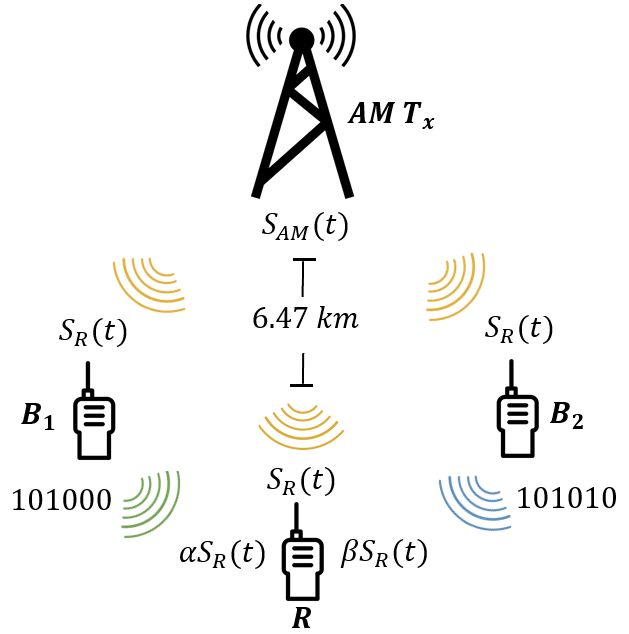
\includegraphics[width=75mm,scale=0.50]{Figure_1.png}}
  \caption{Multipoint-to-point ambient backscatter network with simultaneous transmissions.}
\end{figure}

Moreover, we assume $B_1$, $B_2$, and $R$ have the same high-gain ferrite bar antenna that allows them to receive and reflect the AM signal. We will assume the gain of this antenna, which we denote as $G_A$, is $2.15$ dB. This value is fairly arbitrary and is less than the maximum gain that can be provided by this type of antenna \cite{ferrite_antenna}. $P\{S_{R}(t)\}$ can be estimated as follows:
$$P\{S_{R}(t)\}=P\{S_{AM}(t)\}-FSL+G_A$$
$$P\{S_{R}(t)\}=67 \text{ dBm} - 48.31 \text{ dB} + 2.15 \text{ dBi}$$
$$P\{S_{R}(t)\}\approx 21 \text{ dBm.}$$
As a result of these computations, our model assumes that, at any time instant, $B_1$, $B_2$, and $R$ receive the same 21 dBm AM signal. The values $\alpha$, $0 \leq \alpha \leq 1$, and $\beta$,$0 \leq \beta \leq 1$, represent the attenuation factors of the signals reflected by $B_1$ and $B_2$ with respect to $S_{R}(t)$, respectively, as perceived by $R$.

\section{CONCURRENT TRANSMISSIONS}

Our simulated backscattering transmissions replicate the mechanisms described in  \cite{liu2013ambient}. A device $B_i$, $i \in \{1,2\}$, modulates a series of bits by toggling between reflective and non-reflective states. In real implementations, this switching is performed by modulating the impedance of the antenna such that its reflective properties vary according to the binary input. To transmit a "1" bit, the transmitter enters the backscattering state and reflects the ambient signal it receives. To transmit a "0" bit, it remains idle, i.e., it does not reflect the input signal. In our GNU Radio implementation, concurrent transmissions are modeled according to the following equation:
$$S_{in}(n)= S_{R}(n) + b_{B_1}^\tau(\alpha S_{R}(n)) + b_{B_2}^\tau(\beta S_{R}(n)),$$
where $S_{in}(n)$, $n \in \{1,2,...\}$, is the $n$th sample of the input signal at the receiver, $S_{R}(n)$ is the $n$th sample of the signal received by $R$ from the AM tower, $\alpha$ and $\beta$ are defined as before, $b_{B_1}^\tau \in \{0,1\}$ is the bit transmitted by $B_1$ during the $\tau\text{th}$ bit period, $\tau=\{1,2,3,...\}$, and $b_{B_2}^\tau \in \{0,1\}$ is the bit transmitted by $B_2 $ during the $\tau\text{th}$ bit period. Let $N$ be the number of samples in a bit period. We use a sampling rate of 4.096 MHz and assume that both transmitters communicate at 100 bits/sec. Consequently, each $\tau$ encompasses $N=40,960$ discrete time samples of the signals involved. This equation evinces the four possible states at the receiver:

\begin{itemize}

\item \textbf{Case 1: }During bit period $\tau$, $B_1$ transmits $b_{B_1}^\tau=0$ and $B_2$ transmits $b_{B_2}^\tau=0$. $S_{in}(n)$ is therefore equal to $S_{R}(n)$, i.e., the ambient signal received by $R$ from the AM transmitter.
\item \textbf{Case 2: }During bit period $\tau$, $B_1$ transmits $b_{B_1}^\tau=1$ and $B_2$ transmits $b_{B_2}^\tau=0$. $S_{in}(n)$ is therefore equal to $S_{R}(n) + \alpha S_{R}(n)$, i.e., the ambient signal received by $R$ from the AM transmitter plus the signal $B_1$ backscatters.
\item \textbf{Case 3: }During bit period $\tau$, $B_1$ transmits $b_{B_1}^\tau=0$ and $B_2$ transmits $b_{B_2}^\tau=1$. $S_{in}(n)$ is therefore equal to $S_{R}(n) + \beta S_{R}(n)$, i.e., the ambient signal received by $R$ from the AM transmitter plus the signal $B_2$ backscatters.
\item \textbf{Case 4: }During bit period $\tau$, $B_1$ transmits $b_{B_1}^\tau=1$ and $B_2$ transmits $b_{B_2}^\tau=1$. $S_{in}(n)$ is therefore equal to $S_{R}(n)+ \alpha S_{R}(n) + \beta S_{R}(n)$. In other words, the signal $R$ must process equals the sum of the ambient signal received by $R$ from the AM transmitter, the signal backscattered by $B_1$, and the signal backscattered by $B_2$. 
\end{itemize}

The sampled signal $S_{in}(n)$ is processed by our decoding algorithms, and the objective is to retrieve bits $b_{B_1}^\tau$ and $b_{B_2}^\tau$, $\forall \tau$.


\section{CONCURRENT DEMODULATION}

We propose two procedures to decode simultaneous ambient backscatter transmissions: \textit{Demodulation via Power Superposition} and \textit{Demodulation via Time Offset}. Both demodulation procedures are an extension of the techniques used in \cite{liu2013ambient}. For the $\tau\text{th}$ bit period, the average  is computed as follows:
$$\xi_{\tau}=\frac{1}{N}\sum_{n=1}^{N}|S_{in}(n + N(\tau-1))|^2.$$

\begin{figure}[h!]
  \centerline{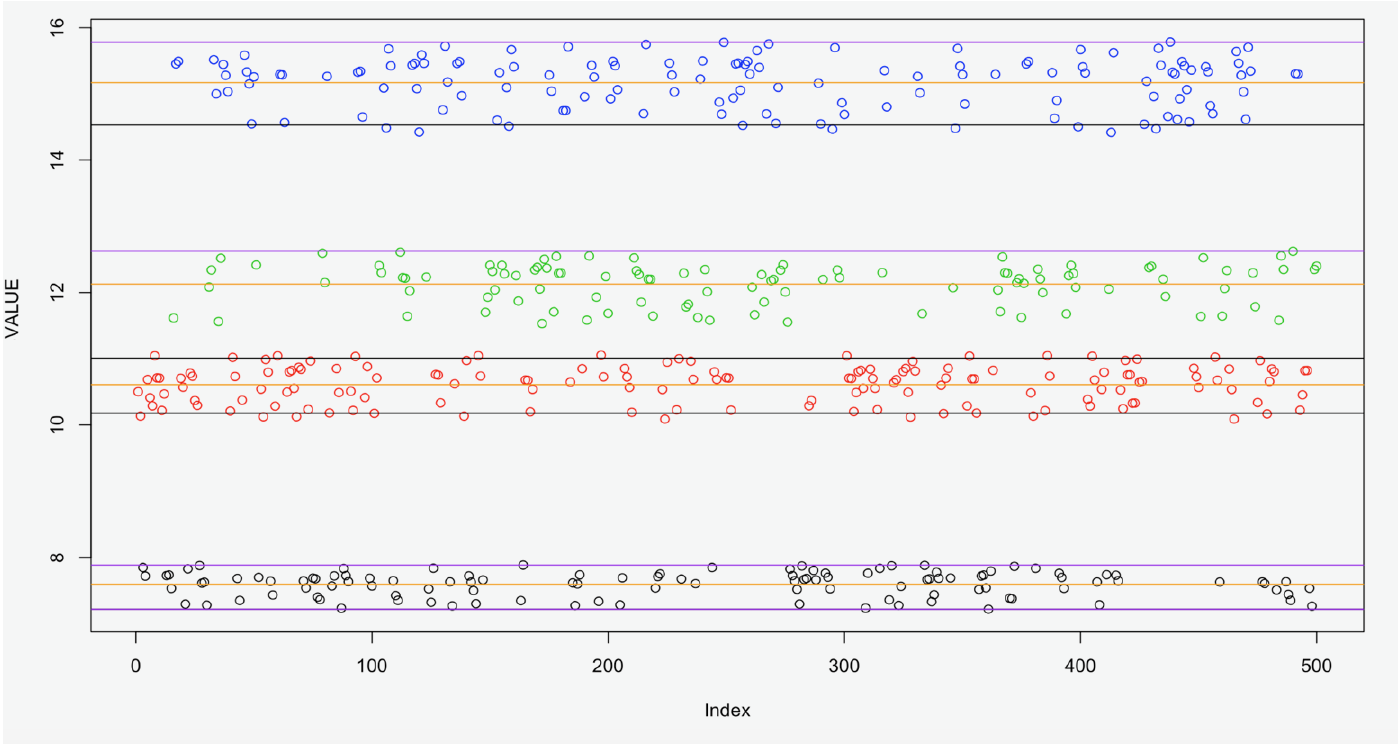
\includegraphics[width=75mm,scale=0.50]{Figure_2.png}}
  \caption{Power levels for several $\xi_{\tau}$.}
\end{figure}
Our decoding schemes analyze in one way or another the sequence of values $\xi_{\tau}$. We argue that, under very special conditions, both proposed mechanisms provide a reliable way to decode concurrent backscatter communications.

\subsection{Demodulation via Power Superposition} The intuition behind this decoding algorithm is that, as long as the difference $|\alpha - \beta|$ is significantly greater than zero at all times during the communication process and it remains consistent, the values $\xi_{\tau}$ will fall predictably above or below 4 very distinctive power levels, one for each of the cases presented before. This effect is shown in Figure 2.

The algorithm starts by initiating a learning process. A sequence of averages $\xi_{1}, \xi_{2}, \xi_{3},...$ is collected for a brief period of time. Assuming $\alpha<\beta$ at all time instances, this sequence is used to compute four thresholds, $T_1<T_2<T_3<T_4$, which are defined as follows:

\begin{figure}[h!]
  \centerline{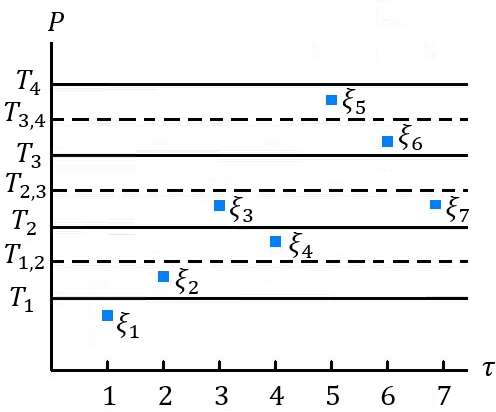
\includegraphics[width=65mm,scale=0.50]{Figure_3.png}}
  \caption{Thresholds used in the Demodulation via Power Superposition algorithm.}
\end{figure}

It is worth pointing out that we assume that the signals always meet constructively at the receiver. Next, the algorithm computes three additional sub-thresholds: $T_{1,2}=\frac{1}{2}(T_1 +T_2)$, $T_{2,3}=\frac{1}{2}(T_2 +T_3)$, $T_{3,4}=\frac{1}{2}(T_3 +T_4)$. Figure 3 shows all the thresholds and possible locations of averages $\xi_{\tau}$. Then, for the $\tau$th bit period, the following decoding process takes place:\\\\if $\xi_\tau \geq T_{3,4}:$\\
\hphantom{1cm}return (1, 1)\\
if $\xi_\tau \geq T_{2,3}$:\\
\hphantom{1cm}return (0, 1)\\
if $\xi_\tau \geq T_{1,2}$:\\
\hphantom{1cm}return (1, 0)\\
return (0, 0)\\\\For instance, $\xi_3$ in Figure 3 indicates that during that bit period, $B_1$ transmitted a "1" bit and $B_2$ transmitted a "0" bit.

We clearly see that for every time period $\tau$, two bits of information are decoded by the receiver, one for each of the transmitters. Hence, this demodulation technique correctly demodulates two transmissions and doubles throughput. Determining the value of $|\alpha - \beta|$ above which demodulation is intractable is beyond the scope of this project. However, by defining this parameter, we can envision a system where more than two backscatterers communicate simultaneously with one receiver.

On the downside, assuming that $|\alpha - \beta|$ will remain consistent during transmission may not be true in practical implementations. The reason is that transmitters can somehow control the power with which they emit a signal, but they can't control the power with which the signal arrives at the receiver. Consequently, if we incorporate exogenous phenomena such as fading and noise in our model, we might not be able to accurately decode bits through power superposition analysis.

\subsection{Demodulation via Time Offset}
The problem with the Power Superposition Demodulation is that it becomes difficult to decode two devices when they transmit at similar power levels. In order to reconcile this problem, we introduce a time offset between the transmissions. Rather than transmitting at the same time, one of the devices will transmit for a time period before the second device begins transmitting. We made this time offset be half of one bit period. After this half bit period, the second device begins transmission, and from here onward the signals are added together to be read at the receiving device.

In order to decode the bit stream, we change our averaging scheme to analyze half of a bit period rather than a full one. At the end of each half period, we average the values over that time. Because of the offset, each half period will represent the start of a new bit period for only one device, alternating between the two devices. In addition to this, the devices will never overlap because they stream bits at the same rate.

As an example, let us assume that $D_1$ is the device that begins transmission first and $D_2$ is the device that begins transmitting after the offset of half of one bit period. The average during the first half period can only be to do $D_1$, because $D_2$ has not started transmitting. When we analyze the average over this period, we know that we can attribute it to $D_1$. In the second half period, any changes in the average must be due to $D_2$, because $D_1$ is in the middle of a bit period and thus cannot change its value. In the third half period, any changes in the average must be due to $D_1$, because it has entered its next bit period, and $D_2$ is in the middle of its previous bit period and cannot change its value. This model continues for the entire bit sequence, and in Figure 4 we can see the changing averages over the half periods, the bit period that the average corresponds to on the x-axis, and below the graph the actual bit being transmitted. 
\begin{figure}[h!]
  \centerline{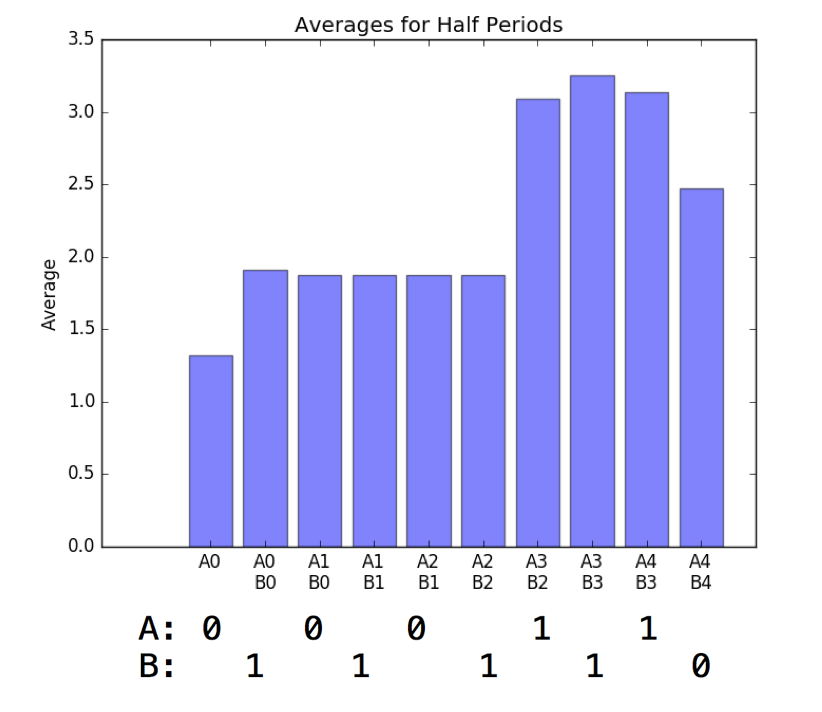
\includegraphics[width=75mm,scale=0.50]{Figure_4.png}}
  \caption{Averages over half periods and the bits they correspond to.}
\end{figure}

Thus, we can use this offset to determine which device is causing a change in the average value received at the receiving device. By alternating between devices after every half window, we know which device has begun a new bit period, and thus which device is causing the change in the average (if any).

To analyze the averages received, we again use the concept of threshold bands to determine changes. We use the same structure as the Power Superposition Model, but we only need bands $T_{1,2}$ and $T_{3,4}$, because we use the offset rather than the power level to determine which device causes changes in the average. If, after a half period, the average goes up a band from the previous period, we know that the device corresponding to that half period is transmitting a 1. If the average goes down a band from the previous average, then we know that it is transmitting a 0. If the average stays within the same band as the previous average, we know that the bit for that device is the same as the last bit it sent, so we reuse its last bit.


 
\section{EVALUATION}

We simulated our scenario of interest using GNURadio in order to test the efficiency of \textit{Demodulation via Power Superposition} and \textit{Demodulation via Time Offset}. 
\begin{figure}[h!]
  \centerline{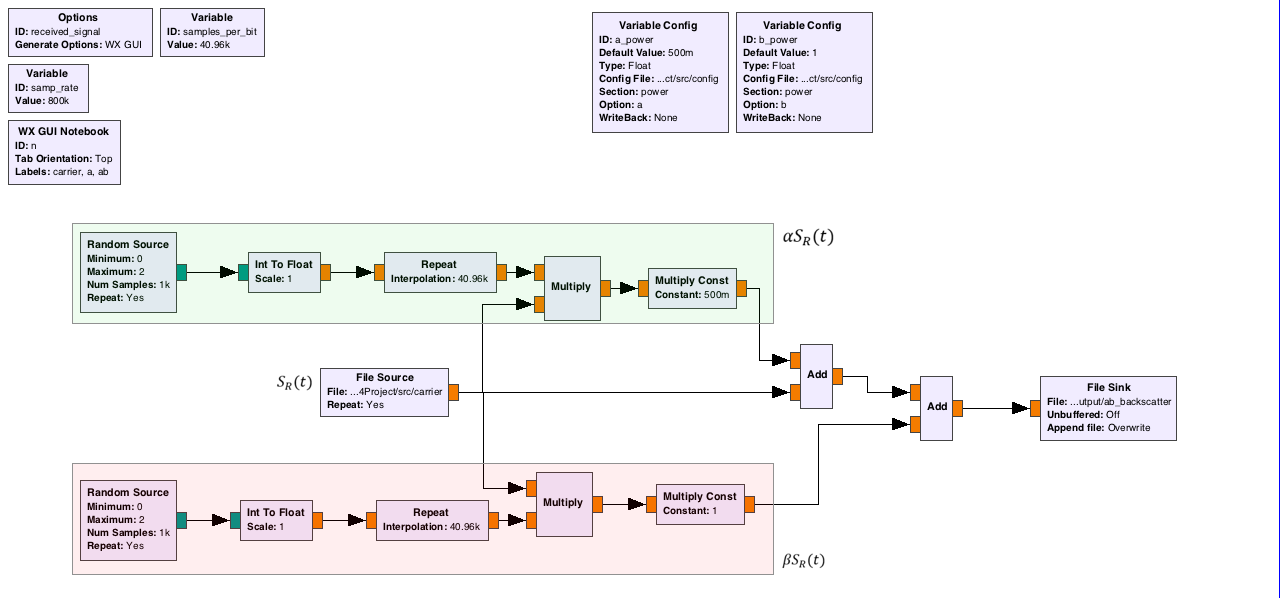
\includegraphics[width=65mm,scale=0.50]{Figure_5(simple).png}}
  \caption{Using GNURadio to build the signal received at R}
\end{figure}

In Figure 4 you can observe that we are constructing the signal by adding the signal $\alpha S_{R}(t)$ if $B_1$ is transmitting a value of 1 or adding 0 otherwise. This is equivalent to creating a new multi-path when $B_1$ is backscattering. We encode the  data for $B_2$ using the same technique with a power level of $\beta$. We began by testing a naive implementation of trying to decode one of the data streams in the presence of two devices transmitting simultaneously. As expected our bit error rate (BER) was steady around 50\% regardless of the power levels of $B_1$ or $B_2$. The single decoder was rendered useless in the presence of a second transmitting device. 

Our implementation of \textit{Demodulation via Power Superposition} doubled the throughput of our channel. As long as the power levels are significantly different, you can encode 4 bits at the same rate that a single transmitter encodes 2 bits. However, there are major limitations to this demodulation technique. First, it lacks scalability. For $n$ devices there are $2^n$ power bands which must all be unique. So although the decoding works well for 2 devices the complexity increases exponentially as the number of devices simultaneously backscattering increases. In addition, the power implementation begins to fail when the bands overlap. Overlapping bands occur in two scenarios:

\begin{itemize}
\item $\alpha = 0$ or $\beta = 0$ If the backscattered signal reaches the receiver with 0 power it is impossible to decode. This happens regardless of the number of devices trying to transmit simultaneously. As such, it is not an issue we will analyze in the paper. 
\item $\alpha = \beta$ In this situation it is impossible to decode the difference between $(1, 0)$ and $(0, 1)$ Figure 6 illustrates an example where $\alpha - \beta$ is close to 0 which causes some points (marked with squares) to be incorrectly decoded. 
\item $\alpha = \beta$. In this situation it is impossible to decode the difference between $(1, 1)$ and $(0, 0)$ \end{itemize}

\begin{figure}[h!]
  \centerline{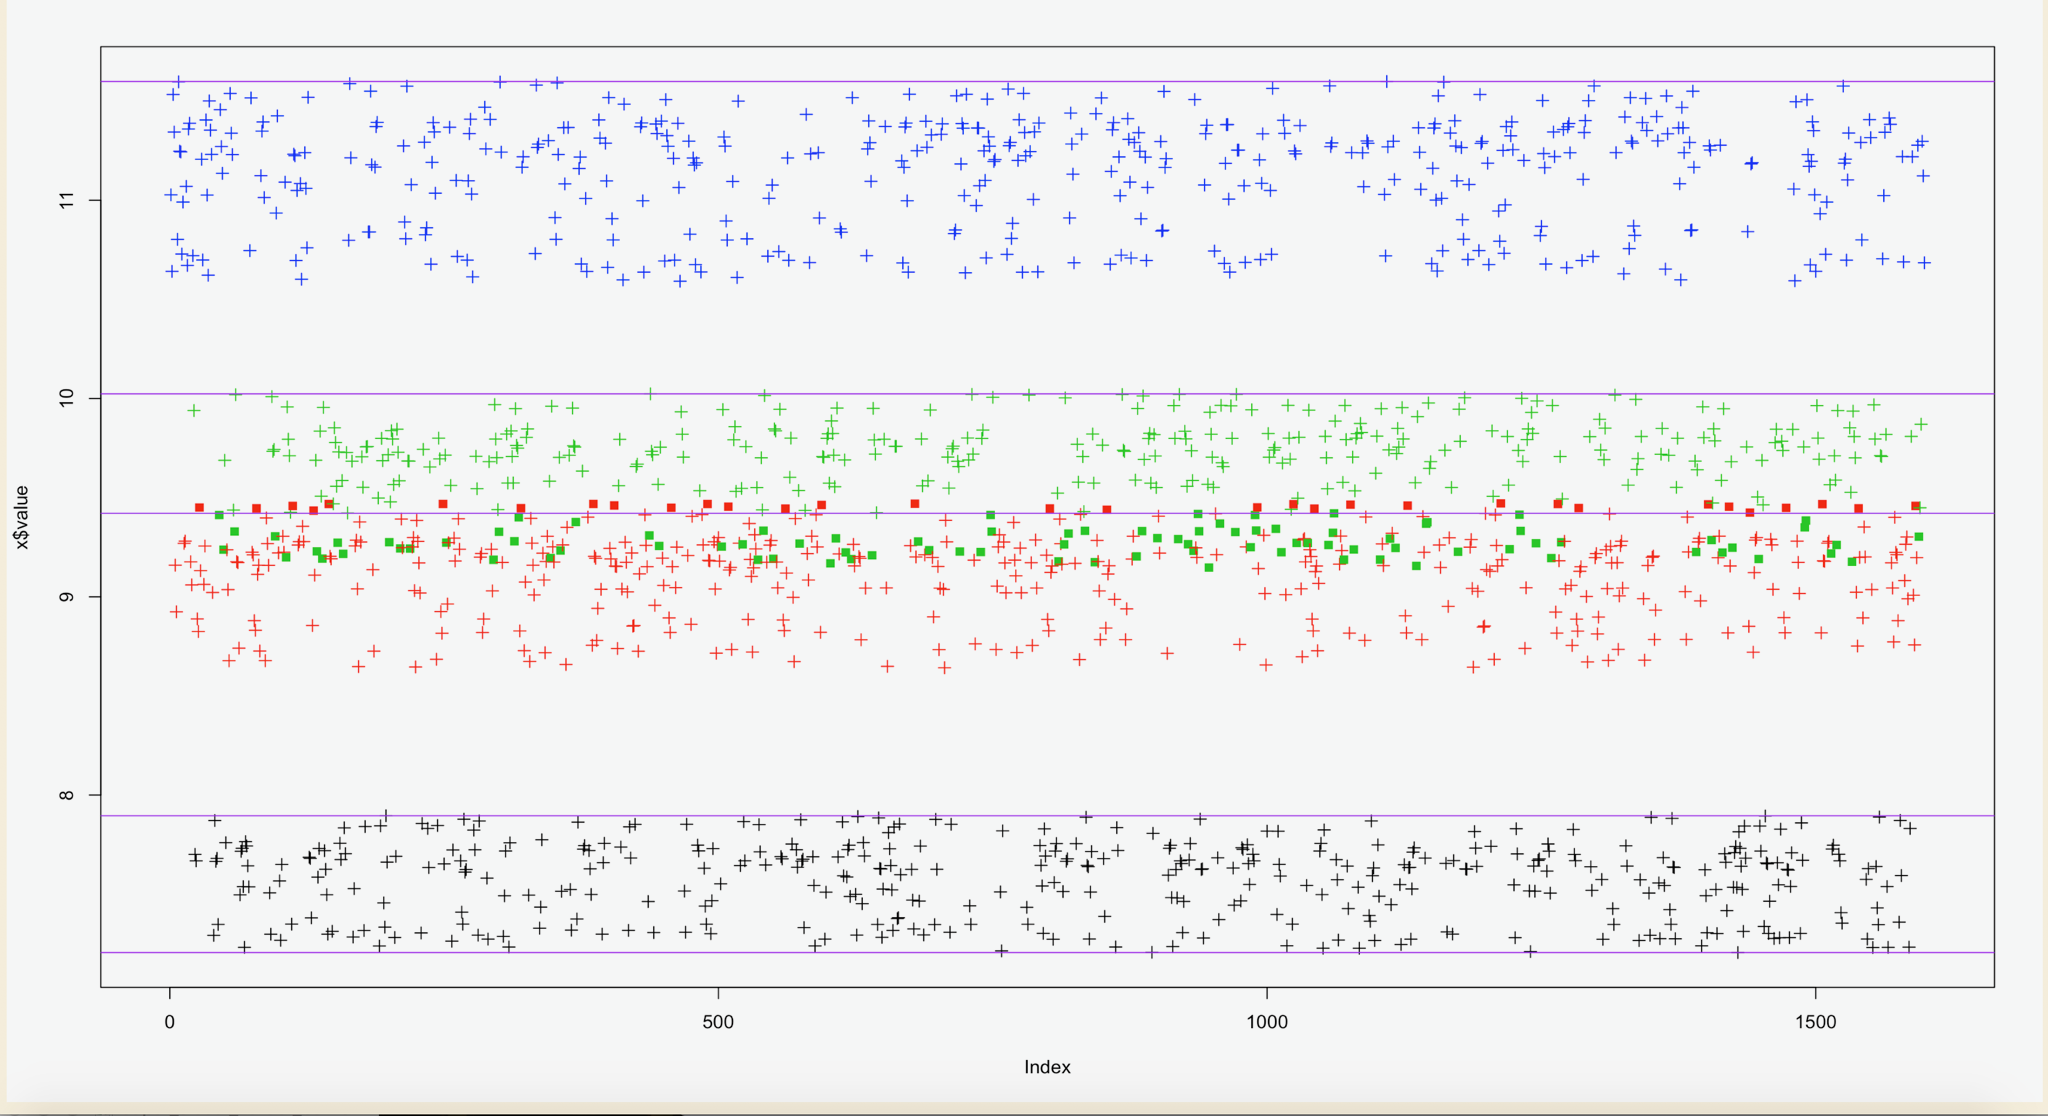
\includegraphics[width=65mm,scale=0.50]{Figure_6.png}}
  \caption{Overlapping power bands cause decoding errors}
\end{figure}

To fully understand the BER of different power levels we fixed $\beta = .5$ and set $0 \leq \alpha \leq 1$ to fluctuate values. The resulting graph (Figure 7) shows 25\% BER centered around 0 when $\alpha = 0$ and around 0.5 when $\alpha = \beta$. This matches our earlier predictions. 

\begin{figure}[h!]
  \centerline{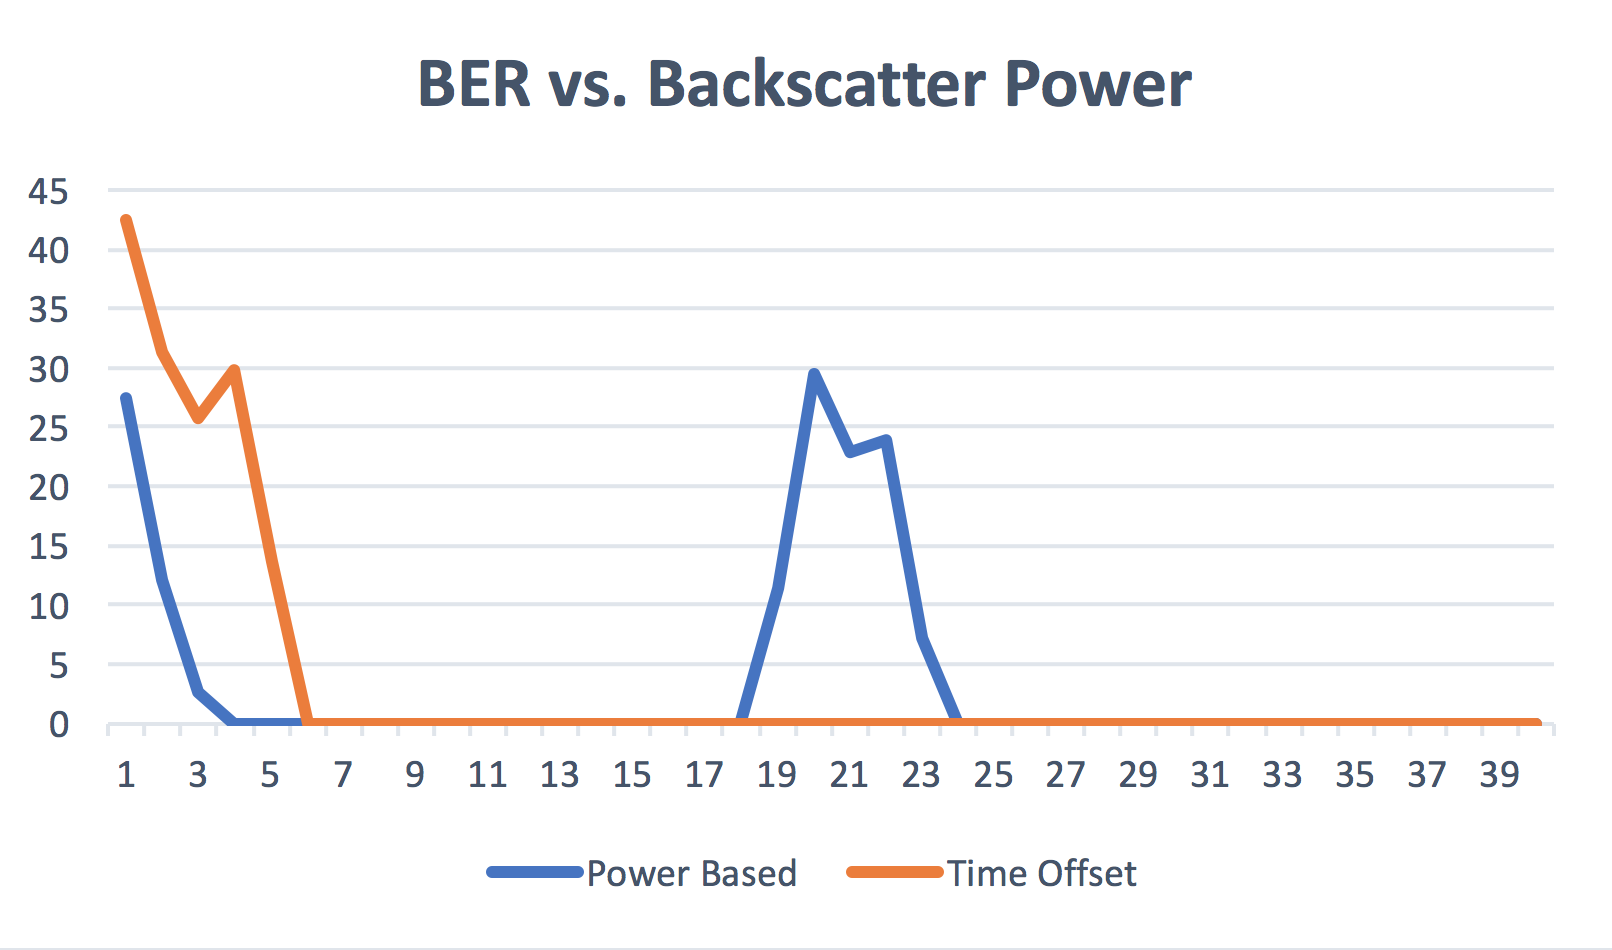
\includegraphics[width=65mm,scale=0.50]{Figure_7.png}}
  \caption{Plotting BER for variable $\alpha$ values}
\end{figure}

Our implementation of \textit{Demodulation via Time Offset} does not double the throughput; however, it still lets two devices transmit simultaneously. 
 \textit{Demodulation via Time Offset} does offer unique advantages over the power based decoding. Primarily, the decoding still works even when $\alpha = \beta$. See Figure 7. Furthermore, this implementation is highly scalable. If backscatter device $B_1$ can transmit at $x$ bits per second, then using our demodulation technique, devices $B_1 \ldots B_n$ can all transmit simultaneously and at $x / n$ bits per second. 

\section{CONCLUSIONS}





\bibliography{biblio}{}
\bibliographystyle{plain}




\end{document}